\documentclass[12pt]{article}

% Packages
\usepackage[utf8]{inputenc}
\usepackage{amsmath, amssymb, amsthm}   % Math
\usepackage{graphicx}           % Images
% \usepackage{hyperref}           % Clickable links
\usepackage{geometry}           % Page margins
% \usepackage{cite}               % Citation formatting
\usepackage{algorithm}
\usepackage{algpseudocode}
\usepackage{listings}
\usepackage{color}

\definecolor{dkgreen}{rgb}{0,0.6,0}
\definecolor{gray}{rgb}{0.5,0.5,0.5}
\definecolor{mauve}{rgb}{0.58,0,0.82}

% BibLaTeX for references (requires biber)
\usepackage[
    backend=biber,
    style=numeric,
    sorting=nyt
]{biblatex}

\addbibresource{references.bib}  % Bib file

% Page setup
\geometry{margin=1in}

% Title
\title{Efficient discrete random variate generation using an entropy store}
\author{Calum Grant \\
OxFORD Asset Management \\
calum.grant@oxam.com}
\date{\today}

\newtheorem{lemma}{Lemma}
\newtheorem{corollary}{Corollary}
\newtheorem{definition}{Definition}
\newtheorem{theorem}{Theorem}

\newcommand{\indep}{\perp\!\!\!\perp}
\newcommand{\unif}[1]{\mathrm{Unif}\{#1\}}
\newcommand{\bern}[1]{\mathrm{Bern}\{#1\}}
\newcommand{\entropy}[1]{\mathrm{H}(#1)}
\newcommand{\prob}[1]{\mathbb{P}(#1)}
\newcommand{\expected}[1]{\mathbb{E}(#1)}

\lstset{
  language=C,        % choose the language
  basicstyle=\ttfamily\small, % font style and size
  keywordstyle=\color{blue},
  commentstyle=\color{gray},
  stringstyle=\color{orange},
  numbers=left,
  numberstyle=\tiny\color{gray},
  stepnumber=1,
  numbersep=5pt,
  showstringspaces=false,
  breaklines=true,
  frame=single,
  captionpos=b
}

\begin{document}

\maketitle

\begin{abstract}
    We present new algorithms for generating discrete random variates from unbiased coins or dice using an \em entropy store \em to improve the entropy efficiency. The method can generate perfect random variates for any weighted integer distribution, whilst losing almost no entropy in the process.  For example we can shuffle a deck of 52 cards using just $\approxeq 225.58102$ bits of entropy, yielding an entropy  efficiency of $\approxeq 0.99999992$ using a 32-bit entropy store, compared with classical algorithms that only have and efficiency of $\approxeq 0.81$. An entropy store allows us to bypass the classical limits on entropy efficiency as established by Knuth and Yao \cite{Knuth1976TheCO}, and has practical applications when generating variates directly from hardware-based entropy which is often a performance bottleneck.    
\end{abstract}

\section{Introduction}

In this paper, we will study generating perfectly distributed integers from an entropy source. A typical example of this is using fair coin flips to roll a fair die or to perform a perfect shuffle of a deck of cards, but random numbers are ubiquitous in other areas such as security, AI, and simulations.

The general problem is one of \em entropy conversion \em, where entropy in one form needs to be converted to entropy in a different form using a function $f$ on a discrete random variable $X$ having Shannon entropy $H(X)$
\cite{shannon1948mathematical}.  
A fundamental result is that you cannot get more entropy out than you put in, or $H(X) \ge H(f(X))$. \cite{cover1999elements} 
We will be mainly focussed on improving the \em efficiency \em of entropy conversion, defined as $\eta = \frac{H(f(X))}{H(X)}$.

Whilst this problem has been studied extensively, there are theoretical limits on efficiency because algorithms must always fetch entropy in units, and any excess entropy is simply lost. An optimal algorithm for generating uniform variables from coin flips must fetch up to 2 extra bits of entropy per output.  \cite{cover1999elements, Knuth1976TheCO}

To mitigate these entropy losses, it is possible to generate random integers in batches. The major drawback with batching schemes is that they do not scale very well and have limits on their capacity and efficiency.

In this paper we will explore a fundamentally different approach, by allowing entropy conversion algorithms access to an \em entropy store \em (ES) in the form of a large uniformly distributed integer, and allow the algorithm to put back any unused entropy into the store. An entropy store allows us to make efficient decisions and recover almost all lost entropy.

The entropy efficiency depends only on the ratio of the size of the store to the size of the number generated, and a precise bound is given in Theorem \ref{thm:loss}. 

For example to roll a 6-sided die with a 32-bit entropy store (holding at least 31 bits of entropy) has an entropy efficiency of $>0.99999997$. To shuffle a deck of 52 cards with a 32-bit entropy store has an entropy efficiency $>0.99999992$. By increasing the size of the store, we can achieve entropy efficiency arbitrarily close to 1.


\subsection {Contribution}

We present new algorithms, called \em entropy store algorithms \em, that have lower setup costs and higher amortised entropy efficiency than classical algorithms. Table \ref{tab:entropy-store} summarises the algorithm, where $m$ is the number of bits in each integer, and $n$ is the size of the weighted distribution. For uniform or Bernoulli outputs, $n=O(1)$. $\epsilon$ is defined in Theorem \ref{thm:loss} and graphed in Figure \ref{fig:uniform-losses}. These characteristics are essentially optimal since $m$ and $n$ are usually constant.  A weighted distribution covers other discrete distribution types such as uniform, rational weights, dyadic and Bernoulli distributions.

\begin{table}[h!]
\centering
\begin{tabular}{|c|c|c|c|c|}
\hline
Input & Output & Entropy & Time & Space \\
\hline
Unbiassed & Weighted & $H(P)+\epsilon$ & Setup: $O(mn)$ & $O(mn)$ \\
coin & Exact & (amortised) & Per output: $O(m \log m)$  &  \\
dice & Markov &  &   & \\
\hline
\end{tabular}
\caption{Entropy store algorithm overview.}
    \label{tab:entropy-store}
\end{table}

No other algorithm has achieved this level of entropy efficiency.

We show that this algorithm outperforms other random number generators when reading directly from a hardware entropy source, where the limiting factor is the rate of entropy input.

\subsection{Related work}

Entropy conversion is a well studied subject going back to at least 1951 when Von Neumann \cite{neumann51} proposed the first known algorithm for generating perfectly uniform variables (a "dice roll") from an unbiassed coin (a "coin flip") - just three years after Claude Shannon's seminal work from 1948 \cite{shannon1948mathematical}. Von Neumann's rejection sampling algorithm works by fetching the smallest power of 2 greater or equal to the number being generated. If the number is in range, return it, otherwise retry. This algorithm is elegant but not optimal in its entropy efficiency.

Knuth and Yao \cite{Knuth1976TheCO} devised an optimal algorithm, based on creating a binary decision tree based on the arithmetic coding of each output, and proved that no other binary decision tree could on average give fewer decisions.

The drawbacks with the original Knuth-Yao algorithm are the setup and space costs: the decision trees are explicitly constructed can get quite large. Lumbruso \cite{lumbroso2013optimal} devised an optimal dice rolling algorithm, that is no more efficient than Knuth-Yao, but requires no setup and is simple to implement. Bacher et al \cite{bacher2017} analyse the Von Neumann and Knuth-Yao algorithms from an entropy perspective, using Lumbruso's implementation, with a particular focus on generating unbiased permutations from unbiased coin flips. There are always up to 2 bits of entropy loss (or 'toll') for each uniform variable generated, depending on the number being generated. Only exact powers of 2 can be generated without entropy loss.

Lemire \cite{lemire2019fast} compares different practical uniform generators, and describes a uniform generator that is efficient from a CPU perspective, but are very inefficient from an entropy perspective, by using fewer CPU division operations. Lemire's use case is for entropy that comes from a pseudorandom source that can be quickly generated.

Various methods have been explored for generating arbitrary intervals.
The Knuth-Yao algorithm can be used to generate arbitrary distributions from binary entropy, but the tree may need to be truncated unless the distribution is dyadic.

XXX My description of the alias method is nonsense and should be revised. XXX

The alias method devised by Walker \cite{walker1977efficient} and improved by Vose \cite{vose91} maps a uniform variable to an arbitrary distribution, and is therefore less entropy efficient because the output distribution generally contains less entropy than the uniform input distribution.

Han and Hoshi \cite{han97} devised an optimal interval algorithm to convert biased or unbiased coin-flips to an arbitrary distribution, with an overhead of up to 3 bits of entropy per output.  The algorithm works by dividing the $[0,1)$ real interval according to the output distribution, and stops at bit n when the fetched binary number falls entirely within the output interval in the nth bit. Han and Hoshi show that this algorithm has an asymptotically optimal entropy consumption. 
Wanatabe \cite{wanatabe20} analyses this algorithm using an information spectrum, and Oohama \cite{oohama11, oohama2020performance} analyses the performance this algorithm.

Saad et al \cite{saad2020fldr} introduce Fast Loaded Dice Roller (FLDR) algorithm and Draper and Saad \cite{draper2025efficient} the Amplified Loaded Dice Roller (ALDR) algorithms to generate more efficient discrete distribution generating trees (DDG). They observe that DDG-based algorithms like Knuth-Yao can be very large and slow, so propose a table-based approach with optimizations, which creates a faster random distribution generator within 2 bits per sample of the output entropy for ALDR, and 6 bits per output for FLDR.

\em Entropy extraction \em studies how to convert the entropy \em from \em a variety of different distributions. When the input distribution is unknown, Von Neumann \cite{neumann51} gives an algorithm to extract unbiased entropy from a biassed coin, which is again elegant but suboptimal in its entropy efficiency. Peres \cite{peres1992iterating} devised a way to recursively use the previously-discarded outputs to provide an algorithm with perfect amortised entropy efficiency, and the method was generalised by Pae \cite{pae15} to extract entropy from arbitrary but identically distributed unknown distributions ("weighted M-dice") with perfect amortised efficiency. Interestingly, it appears to be easier to extract entropy than to generate it.

Universal hashing can be used to turn unknown distributions into fair bits. Vembu et al \cite{vembu95} analyse the maximum rate at which entropy can be extracted. Goldreich's Leftover hash lemma \cite{goldreich2004foundations} calculates the length of possible output. Trevisan \cite{trevisan2001extractors} implements a universal hash extractor for unknown distributions with a known entropy. 

A common proposal to reach asymptotic efficiency for random number generation is to use batching to generate multiple outputs at the same time. \cite{bacher2017,han97,devroye86,Knuth1976TheCO,lumbroso2013optimal} Batching spreads the entropy loss over the batch size. However batching schemes suffer from increased size and complexity, and are less flexible because you must plan beforehand which numbers to generate. The fundamental limit to batching is that they do not scale well because they require arbitrary output precision or data structure sizes.

Fill and Huber \cite{fill2000randomness, huber2016perfect}, describe the \em randomness recycler \em protocol which is a general purpose strategy to identify excess entropy in an algorithm and store it for the next state. This ideas has been used to generate entropy-optimal uniform \cite{lumbroso2013optimal, huber2024optimal} or weighted \cite{huber2024optimal} variables, but only within a single output, so does not improve on the efficiency established by Knuth-Yao and Han-Hoshi.


\section{Algorithms for entropy conversion}

In this section we'll start with some basic building blocks (Algorithm \ref{alg:combine}-\ref{alg:generate-multiple}), and then use these to create an efficient generator for uniform variables (Algorithm \ref{alg:generate-uniform}).

We'll then build on Algorithm \ref{alg:generate-multiple} to create a generator for Bernoulli variables (Algorithm \ref{alg:generate-bernoulli}) and weighted distributions (Algorithm \ref{alg:generate-weighted}). All of these algorithms are designed to have a 1 or near-1 entropy efficiency, and proofs of correctness and efficiency are contained throughout this section.

We'll use uppercase letters $X$, $Y$ and $Z$ for discrete random variables, and write $\entropy{X}$ for the Shannon entropy of this variable. Write $X \sim \unif{0..n-1}$ to mean that $X$ has a uniform variable distribution of "size" $n$, or $X \sim \unif{n}$ for short, because all uniform distributions will be 0-based. $\entropy{\unif{n}} = \log_2n$. The interval $[a,b)$ means all integers in the range $a...b-1$. Write $\mathbb{P}$ for probability, $\mathbb{E}$ for expected value, and lowercase $f$ as a function on random variables. $f^{-1}$ means the inverse function. $A \indep B$ means that random variables $A$ and $B$ are independent. In algorithms, $\div$ and $\mod$ are integer division and modulus operations, and subscripts are implemented as array access.

We'll say "uniform variable" to mean a uniformly distributed integer variable or variate.


\subsection{Basic operations}

At the basis of the ES is the ability to transform a uniform variable into different forms.  We can divide a uniform variable into (a) two uniform variables, (b) a Bernoulli variable and a uniform variable, (c) a weighted variable and a uniform variable. These transformations are bijective, meaning they preserve entropy, and can be used in both directions. Similar ideas can be found for example in \cite{gentle2003random} Ch. 4 (XXX check this), and we are simply writing these as algorithms. The contribution is how we combine these mappings for entropy conversion.

The function $f_{combine}$, in Definition \ref{def:combine}, allows us two combine two uniform variables $X$ and $Y$ into a single uniform variable $Z$. Its inverse $f^{-1}_{combine}$ in given in Lemma \ref{lem:divide}. $f_{combine}$ and $f^{-1}_{combine}$ divide an interval of size $nm$ into $n$ intervals of size $m$ as follows:


\[
\overbrace{
        \underbrace{a_0 ... a_{m-1}}_{m}
        \underbrace{a_m ... a_{2m-1}}_{m}
        ...
        \underbrace{a_{n(m-1)}...a_{nm-1}}_{m} 
        }
        ^{nm}
\]

\begin{definition}
    $f_{combine}: [0,n)\times [0,m) \rightarrow [0,nm)$ is defined as $f_{combine}(X,Y) = mX+Y$.
    \label{def:combine}
\end{definition}

\begin{lemma}
    $f_{combine}$ is a bijection with inverse $f^{-1}_{combine}(Z) = (\lfloor \frac{Z}{m} \rfloor, Z \mod m)$.
    \label{lem:divide}
\end{lemma}

\begin{proof}
    $f_{combine}(f^{-1}_{combine}(Z)) = f_{combine}(\lfloor \frac{Z}{m}\rfloor, Z \text{ mod } m) = m(\lfloor \frac{Z}{m}m \rfloor) + (Z \mod m) = Z$. $f^{-1}_{combine}(f_{combine}(X,Y)) = f^{-1}_{combine}(mX+Y) = (\lfloor\frac{mX+Y}{m}\rfloor, (mX+Y)\mod m) = (X,Y)$. Therefore $f_{combine}$ is a bijection.
\end{proof}

\begin{lemma}
    If $X \sim \unif{n}$ and $Y \sim \unif{m}$ and $X \indep Y$, then 
    $f_{combine}(X,Y) \sim \unif{nm}$.
\end{lemma}

\begin{proof}
    Let $Z = mX+Y$, so $Z \in [0,nm)$. $\prob{X=x,Y=y} = \prob{X=x}\mathbb{P}(Y=y) = \frac{1}{n}\frac{1}{m} = \frac{1}{nm}$. Since $f_{combine}$ is a bijection then it means that all $z$ values occur with $\prob{Z=z} = \frac{1}{nm}$, so $Z \sim \unif{nm}$.
    
\end{proof}

\begin{lemma}
    If $Z \sim \unif{nm}$, and $f^{-1}_{combine}(Z) = (X,Y)$, then $X \sim \unif{n}$ and $Y \sim \unif{m}$. $X \indep Y$.
    \label{lem:combine-independent}
\end{lemma}

\begin{proof}
    $\prob{X=x,Y=y} = \frac{1}{nm}$. $\prob{X=x} = \sum_{y}\prob{X=x,Y=y} = m\frac{1}{nm} = \frac{1}{n}$. $\prob{Y=y} = \sum_{x}\prob{X=x,Y=y} = n\frac{1}{nm} = \frac{1}{m}$. Therefore $X\sim \unif{n}$ and $Y\sim \unif{m}$.

    $\mathbb{P}(X=x,Y=y) = \frac{1}{nm} = \mathbb{P}(X=x)\mathbb{P}(Y=y)$, so $X \indep Y$.
\end{proof}

Algorithm \ref{alg:combine} is an implementation of $f_{combine}$, and Algorithm \ref{alg:divide} is an implementation of $f^{-1}_{combine}$. Algorithm \ref{alg:combine} will be used to \em add \em entropy to the entropy store, and Algorithm \ref{alg:divide} can be used to \em extract \em entropy from the entropy store.

\begin{algorithm}
\caption{Combining two uniform variables into one uniform variable}
\label{alg:combine}
\begin{algorithmic}[1]
    \Require $N, M, n$ and $m$ are integers
    \Require $N \sim \unif{n}$
    \Require $M \sim \unif{m}$
    \Require $N \indep M$
    \Ensure $s$ is $n * m$
    \Ensure $S \sim \unif{s}$
\Procedure{combine}{$N, n, M, m$} 
  \State $S \gets N * m + M$
  \State $s \gets n * m$
  \State \Return $S, s$
\EndProcedure
\end{algorithmic}
\end{algorithm}

\begin{algorithm}
\caption{Converting a uniform variable into two uniform variables by division}
\label{alg:divide}
\begin{algorithmic}[1]
    \Require $S, s$ and $n$ are integers
    \Require $s \mod m = 0$, i.e. $s$ is divisible by $m$
    \Require $S \sim \unif{s}$
    \Ensure $n * m = s$
    \Ensure $N \sim \unif{n}$
    \Ensure $M \sim \unif{m}$
    \Ensure $N \indep M$
\Procedure{divide}{$S, s, m$} 
  \State $N \gets S \div m$
  \State $M \gets S \mod m$
  \State $n \gets s \div m$
  \State \Return $N, n, M$
\EndProcedure
\end{algorithmic}
\end{algorithm}


The function $f_{sample}$, in Definition \ref{def:sample}, divides the range $[0,n)$ into two parts:

\[
\overbrace{
    \underbrace{
        \underbrace{a_0 \text{   } ... \text{   } a_{m-1}}_{m}
        \underbrace{a_m \text{   } ... \text{   } a_{n-1}}_{n-m}}
    }_{\bern{\frac{m}{n}}}^{n}
\]

\begin{definition}
$f_{sample}: [0,n) \rightarrow \{0,1\} \times [0,\max(n,n-m))$ is defined as $f_{sample}(Z) = (Z<m, m(Z\ge m) + Z)$. (Assume that the operators $<$ and $\ge$ evaluate to $0$ or $1$.)
\label{def:sample}
\end{definition}

\begin{lemma}
If $Z \sim \unif{n}$ and $f_{sample}(Z) = (X,Y)$, then $X \sim \bern{\frac{m}{n}}$ and $Y \sim \unif{m(Z \ge m)+Z}$. $X \indep Y$.
\end{lemma}

\begin{proof}
    ...
\end{proof}

Algorithm \ref{alg:sample} implements $f_{sample}$. Algorithm \ref{alg:sample} can be used to resize a uniform distribution or to generate a Bernoulli variable.


\begin{algorithm}
\caption{Converting a uniform variable into a Bernoulli and a uniform variable}
\label{alg:sample}
\begin{algorithmic}[1]
    \Require $N, n$ and $m$ are integers 
    \Require $0 \le m \le n$
    \Require $N \sim \unif{n}$
    \Ensure $B \sim \bern{\frac{m}{n}}$
    \Ensure $X \sim \unif{x}$
    \Ensure $x = Bm + (1-B)(n-m)$
    \Ensure $X \indep B$
\Procedure{sample}{$N, n, m$} 
  \If{$N < m$}
    \State $B \gets 1$  
    \State $x \gets m$
    \State $X \gets N$
  \Else
    \State $B \gets 0$  
    \State $x \gets n-m$
    \State $X \gets N-m$
  \EndIf
  \State \Return $X, x, B$
\EndProcedure
\end{algorithmic}
\end{algorithm}

\begin{lemma}
    $f_{sample}$ preserves entropy.
\end{lemma}

\begin{proof}
    ...
\end{proof}

Algorithms \ref{alg:combine} and \ref{alg:sample} appear as building blocks in von Neumann's rejection sampling algorithm and Lumbrusco's FDR algorithm. The reason why rejection sampling and FDR lose entropy is because they discard one or both outputs from the $\textsc{sample}()$ algorithm.



\subsection{Generating uniform variables using an entropy store}

The basis of generating uniform variables (and other distributions) is to obtain a uniform variable $S \sim \unif{s'n}$ where $n$ is the number you need to generate, and $s'$ is an integer. Then we use $\textsc{divide}$ (Algorithm \ref{alg:divide}) to split $\unif{s'n}$ into $\unif{s'}$ and $\unif{n}$, as shown in Algorithm \ref{alg:generate-uniform}. $\unif{n}$ is our result, and $S' \sim \unif{s'}$ is the new entropy store.

Creating $\unif{s'n}$ from an arbitrary entropy store $\unif{s}$ is much easier than it sounds, because you just call $\textsc{sample}(S, s, s - s \mod n)$, which most of the time will return a uniform variable $\unif{s'n}$ (and the other time, $\unif{s \mod n}$).

Algorithm \ref{alg:generate-multiple} is used to generate a uniform variable $\sim \unif{kn}$, by combining binary or uniform entropy into an existing store (line 4) until it reaches a minimum size $s_{min}$ (line 3). Then it resizes $S$ to be a multiple of $n$ on line 8, and if successful, returns the result on line 10. If it fails ($B$ is false), then repeat. The reason this is efficient is because it is overwhelmingly likely that $B$ is true, and so the lost entropy contained in $B$ is very small.

A C implementation of Algorithm \ref{alg:generate-uniform} is given in Appendix \ref{app:source-code}.

\begin{algorithm}
\caption{Generating a uniform round multiple}
\label{alg:generate-multiple}
\begin{algorithmic}[1]
\Require $S, s, s_{min}, n$ and $b$ are integers
\Require $n \le s_{min}$
\Require $b \ge 2$
\Require $\textsc{fetch}() \sim \unif{b}$
\Require $S \sim \unif{s}$
\Ensure $S \sim \unif{kn}$
\Procedure{generate\_multiple}{$S, s, n$} 
  \While {True}
    \While {$s < s_{min}$}
        \State $S, s \gets \textsc{combine}(S, s, \textsc{fetch}(), b)$
    \EndWhile
    \State $k \gets s \div n$
    \State $r \gets s \mod n$
    \State $S, s, B \gets \textsc{sample}(S, s, s-r)$ 
    \If{$B$}
        \State \Return $S, s, k$
    \EndIf
  \EndWhile
\EndProcedure
\end{algorithmic}
\end{algorithm}

\begin{algorithm}
\caption{Generating a uniform variable of a given size}
\label{alg:generate-uniform}
\begin{algorithmic}[1]
\Require $S, s$ and $n$ are integers
\Require $S \sim \unif{s}$
\Ensure $N \sim \unif{n}$
\Ensure $S \sim \unif{s}$
\Ensure $S \indep N$
\Procedure{generate\_uniform}{$S, s, n$} 
  \State $S, s, k \gets \textsc{generate\_multiple}(S, s, n)$
  \State $S, s, N \gets \textsc{divide}(S, s, n)$
  \State \Return $S, s, N$
\EndProcedure
\end{algorithmic}
\end{algorithm}

\begin{lemma}
    In Algorithm \ref{alg:generate-uniform}, 
$N \sim \unif{n}$ and $S \sim \unif{s}$.
\end{lemma}

\begin{proof}
The values $U_n$, $n$, $U_s$ and $s$ have been generated by Algorithms \ref{alg:combine}, \ref{alg:divide} and \ref{alg:sample}. By Lemmas \ref{lem:combine}, \ref{lem:divide} and \ref{lem:sample}, $U_n$ and $U_s$ are uniformly distributed.
\end{proof}

Algorithm \ref{alg:generate-multiple} terminates with probability 1.

\begin{lemma}
    \label{lem:shannon-inequality}

For $p,q \in \mathbb{R}$, where $0 \le p\le q \le 0.5$, 

\begin{equation}
-p\log_2 p - (1-p)\log_2(1-p) \le -q\log_2 q - (1-q)\log_2(1-q)
\end{equation}
\end{lemma}

\begin{proof}
    Let
    \begin{align}
        g(p) & = -p\log_2 p - (1-p)\log_2(1-p) \\
        \implies g'(p) & = \log_2\frac{1-p}{p} = \log_2(\frac{1}{p}-1) \ge \log_21 = 0 
    \end{align}
Since the derivative of $g>0$ it means that $g$ is monotonic.
\end{proof}

\begin{definition}
    Let $\epsilon = \epsilon(p)$ be the expected entropy loss function of Algorithm \ref{alg:generate-uniform}, where $p=\frac{n-1}{s_{min}}$.
\end{definition}

\begin{theorem}
    \label{thm:loss}
If $p = \frac{n-1}{s_{min}} < 0.5$, then

\begin{equation}
0 \le \epsilon(p) \le -\frac{p}{1-p}\log_2p - \log_2(1-p)
\end{equation}

\end{theorem}

\begin{proof}
For each iteration $i$ of Algorithm \ref{alg:generate-uniform}, let $p_i = \frac{s_i \mod n}{s_i}$. But $(s_i \mod n) \le n-1$ and $s_i \ge s_{min}$, so $\frac{s_i \mod n}{s_i} \le \frac{n-1}{s_{min}}$, so $p_i \le p$. On each iteration, the entropy lost is equal to the entropy in the variable $b_i \sim Bernoulli\{p_i\}$, which is given by the entropy equation for a Bernoulli distribution \cite{cover1999elements}:

\begin{equation}
H(b_i) = -p_i\log_2p_i - (1-p_i)\log_2(1-p_i)
\end{equation}

Therefore, 

\begin{equation}
0 \le H(b_i) \le -p\log_2p - (1-p)\log_2(1-p) 
\end{equation}

by Lemma \ref{lem:shannon-inequality}. The expected number of iterations $m$ is given by

\begin{align}
& m = 1 + p_im \le 1 + pm \\
\implies & m-pm \le 1 \\
\implies & m(1-p) \le 1 \\
\implies & m \le \frac{1}{1-p}
\end{align}

The total entropy lost by the algorithm is given by the number of iterations of the algorithm multiplied by the entropy lost in each iteration.

\begin{align}
0 \le m\entropy{b_i} \le & \frac{1}{1-p}(-p\log_2p - (1-p)\log_2(1-p) ) \\
= & -\frac{p}{1-p}\log_2p - \log_2(1-p)
\end{align}

We can also end up in the situation where $(s \mod n) = 0$ already, in which the \em sample \em step always succeeds with no entropy loss, so $\epsilon=0$.
\end{proof}

The actual entropy loss incurred by Algorithm \ref{alg:generate-uniform} depends on whatever values are found in $U_s$ and $s$, so we can only give an upper bound.

\begin{corollary}
The entropy efficiency $\eta$ of Algorithm \ref{alg:generate-uniform} is bounded by

\begin{equation}
\frac{\log_2n}{\log_2n + \epsilon(\frac{n-1}{s_{min}})} \le \eta \le 1
\label{eq:generate-uniform-efficiency}
\end{equation}
\end{corollary}

\begin{proof}
\begin{align}
    \eta & = \frac{H_{out}}{H_{in}} \\
         & = \frac{H_{out}}{H_{out}+\epsilon} \\
         & = \frac{\log_2n}{\log_2n + \epsilon(\frac{n-1}{s_{min}})}
\end{align}
Therefore 
\begin{equation}
\frac{\log_2n}{\log_2n + \epsilon(\frac{n-1}{s_{min}})} \le \eta \le 1
\end{equation}
from Theorem \ref{thm:loss}.
\end{proof}

To illustrate Equation \ref{eq:generate-uniform-efficiency}, if $s_{min}=2^{31}$ and $n=6$, then $\eta \ge 0.99999997$. This means that even with a modest entropy buffer, we can get very good entropy efficiency.

\begin{corollary}
The entropy efficiency $\eta$ of Algorithm \ref{alg:generate-uniform} is arbitrarily close to 1.
\end{corollary}

\begin{proof}
$\epsilon(\frac{n-1}{s_{min}}) \rightarrow 0$ as $s_{min} \rightarrow \infty$, using L'H\^opital's Rule. Therefore $\eta \rightarrow 1$ as $s_{min} \rightarrow \infty$.
\end{proof}



\subsection{Generating Bernoulli variables}

\begin{algorithm}
\caption{Generating a Bernoulli variable}
\label{alg:generate-bernoulli}
\begin{algorithmic}[1]
\Require $S, s, m, n$ are integers
\Require $S \sim \unif{s}$
\Require $0 \le m \le n\le s_{min}$
\Ensure $B \sim \bern{\frac{m}{n}}$
\Ensure $S \sim \unif{s}$
\Ensure $S \indep B$
\Procedure{generate\_bernoulli}{$S, s, m, n$} 
  \State $S, s, k \gets \textsc{generate\_multiple}(U_s, s, n)$
  \State $S, s, B \gets \textsc{sample}(U_s, s, k * m)$
  \State \Return $S, s, B$
\EndProcedure
\end{algorithmic}
\end{algorithm}


\subsection{Generating weighted integer variables}

Algorithm \ref{alg:generate-distribution} shows how we can generate an arbitrary  distribution of $k$ outcomes where each outcome has integer weight $\{w_0, w_1, ..., w_{k-1}\}$, normalised to a discrete distribution with probabilities $\{\frac{w_0}{n}, \frac{w_1}{n}, ..., \frac{w_{k-1}}{n}\}$ where $n=\sum_i w_i$ is the total weight.

The algorithm works by constructing a surjective mapping from the $n$ outcomes of a uniform distribution to the $k$ outputs of the weighted distribution. This uses a simple lookup table of size $n$, constructed using Algorithm \ref{alg:generate-lookup-tables}. If $n$ is very large we could implement the mapping as a binary search on $offset$ instead. To generate an output, call $generate\_uniform$ to generate a integer in the range $[0,n)$, and use the number in the $output$ lookup table as the result. 

We would expect this process to lose entropy because in general the output distribution contains less entropy than the input distribution. The new idea is that we can recover all of the entropy from this process. By splitting up $[0,n)$ into chunks of size $w_i$, each value in $[0,n)$ is contained in a uniform distribution $\unif{w_i}$.

\[
\overbrace{
    \underbrace{
        \underbrace{a_0 ... a_{w_0-1}}_{w_0}
          \underbrace{a_{w_0} ... a_{w_0+w_1-1}}_{w_1}
          ...
          \underbrace{
             a_{n-w_{k-1}} ... 
             a_{n-1}
         }_{w_{k-1}}
    }_{Weighted\{w_0, ..., w_{k-1}\}}
}^{n}
\]

The chunk contains $\log_2w_i$ entropy. We can use $combine$ to return this entropy back to the entropy store. Lemma \ref{lem:distribution-conservation} shows us that when we account for this extra entropy then no entropy is lost.



\begin{definition}
    Let $f_{distribute}: X \rightarrow Y, Z$ be the function that maps random variable $X \sim \unif{n}$ to independent random variables $Y$ and $Z \sim \unif{w_i}$.

    \begin{align}
    Y &= max(j : \sum_{i<j}w_i<X) \\
    Z &= X - \sum_{i<Y}w_i
    \end{align}

\end{definition}

Note that $f_{distribute}$ is a generalisation of XX $f_{combine}$ and $f_{sample}$ XX we didn't define $f_{sample}$.

\begin{lemma}
    \label{lem:distribution-conservation}
    $f_{distribute}$ does not lose entropy
\end{lemma}

\begin{proof}
    \begin{align}
    \mathbb{E}(H(X)) & = \log_2 n \\
    \mathbb{E}(H(Y) + H(Z)) &=  \mathbb{E}(H(Y)) + \mathbb{E}(H(Z)) \\
               & = - \sum_i p_i \log_2p_i + \sum_i p_iH(Y|X=i) \\
               & = - \sum_i \frac{w_i}{n} \log_2 \frac{w_i}{n} + \sum_i \frac{w_i}{n}\log_2 w_i \\
               & = - \sum_i \frac{w_i}{n}(\log_2 w_i - \log_2 n) + \sum_i \frac{w_i}{n}\log_2 w_i \\
               & = - \sum_i \frac{w_i}{n}\log_2 w_i + \sum_i \frac{w_i}{n} \log_2 n + \sum_i \frac{w_i}{n}\log_2 w_i \\
               & = \sum_i \frac{w_i}{n} \log_2 n \\
               & = \frac{\log_2 n}{n} \sum_i w_i \\
               & = \frac{\log_2 n}{n} n \\
               & = \log_2 n
    \end{align}
\end{proof}

\begin{algorithm}
\caption{Generating a weighted variable}
\label{alg:generate-weighted}
\begin{algorithmic}[1]
\Require $S, s$ and $n$ are integers
\Require An array $w$ of $n$ integer weights $w_i \ge 0$
\Require An array $o$ of $n$ integer offsets $o_0 = 0$, $o_{i+1} = o_i + w_i$
\Require An array $p$ of $\sum_i w_i$ integer outputs $p_j = i$ for $o_i \le j < o_{i+1}$
\Require $S \sim \unif{s}$
\Ensure $S \sim \unif{s}$
\Ensure $W \sim Weighted\{w\}$
\Ensure $S \indep W$
\Procedure{generate\_weighted}{$S, s, n, w, p, o$} 
    \State $S, s, k \gets \textsc{generate\_multiple}(S, s, n)$
    \State $W \gets p_{[S \div k]}$
    \State $s \gets k * w_{[W]}$
    \State $S \gets S - o_{[W]}$ 
    \State \Return $S, s, W$
\EndProcedure
\end{algorithmic}
\end{algorithm}

\begin{lemma}
The inverse of $f_{distribute}$ is given by

    \begin{equation}
    f^{-1}_{distribute}(Y,Z) = \sum_{i<Y}w_i + Z
    \end{equation}
\end{lemma}

\begin{proof}
    Show that $f^{-1}f= I$

\end{proof}




\section {Evaluation}

We can evaluate a random number generator based on its speed, memory footprint, setup time, entropy efficiency and quality of output distribution. \cite{saad2025}

For entropy efficiency, we can compare entropy-store (ES) against entropy-optimal algorithms Knuth-Yao (KY) and the Interval Algorithm (IA).

Figure \ref{fig:uniform-losses} shows the calculated entropy loss for generating uniform variables, comparing ES with von Neumann and Knuth-Yao generators. Consistent with theory, the entropy loss of von Neumann and Knuth-Yao generators depend on the number generated, with Knuth-Yao losing up to 2 bits per output.

This figure shows the entropy loss calculated using Equation \ref{eq:generate-uniform-efficiency} for a 32-bit and a 64-bit entropy buffer, with an increase in buffer size yielding a higher efficiency. We can also show sample real-world entropy losses confirming that Equation \ref{eq:generate-uniform-efficiency} is an upper bound.

\begin{figure}[ht]
\centering
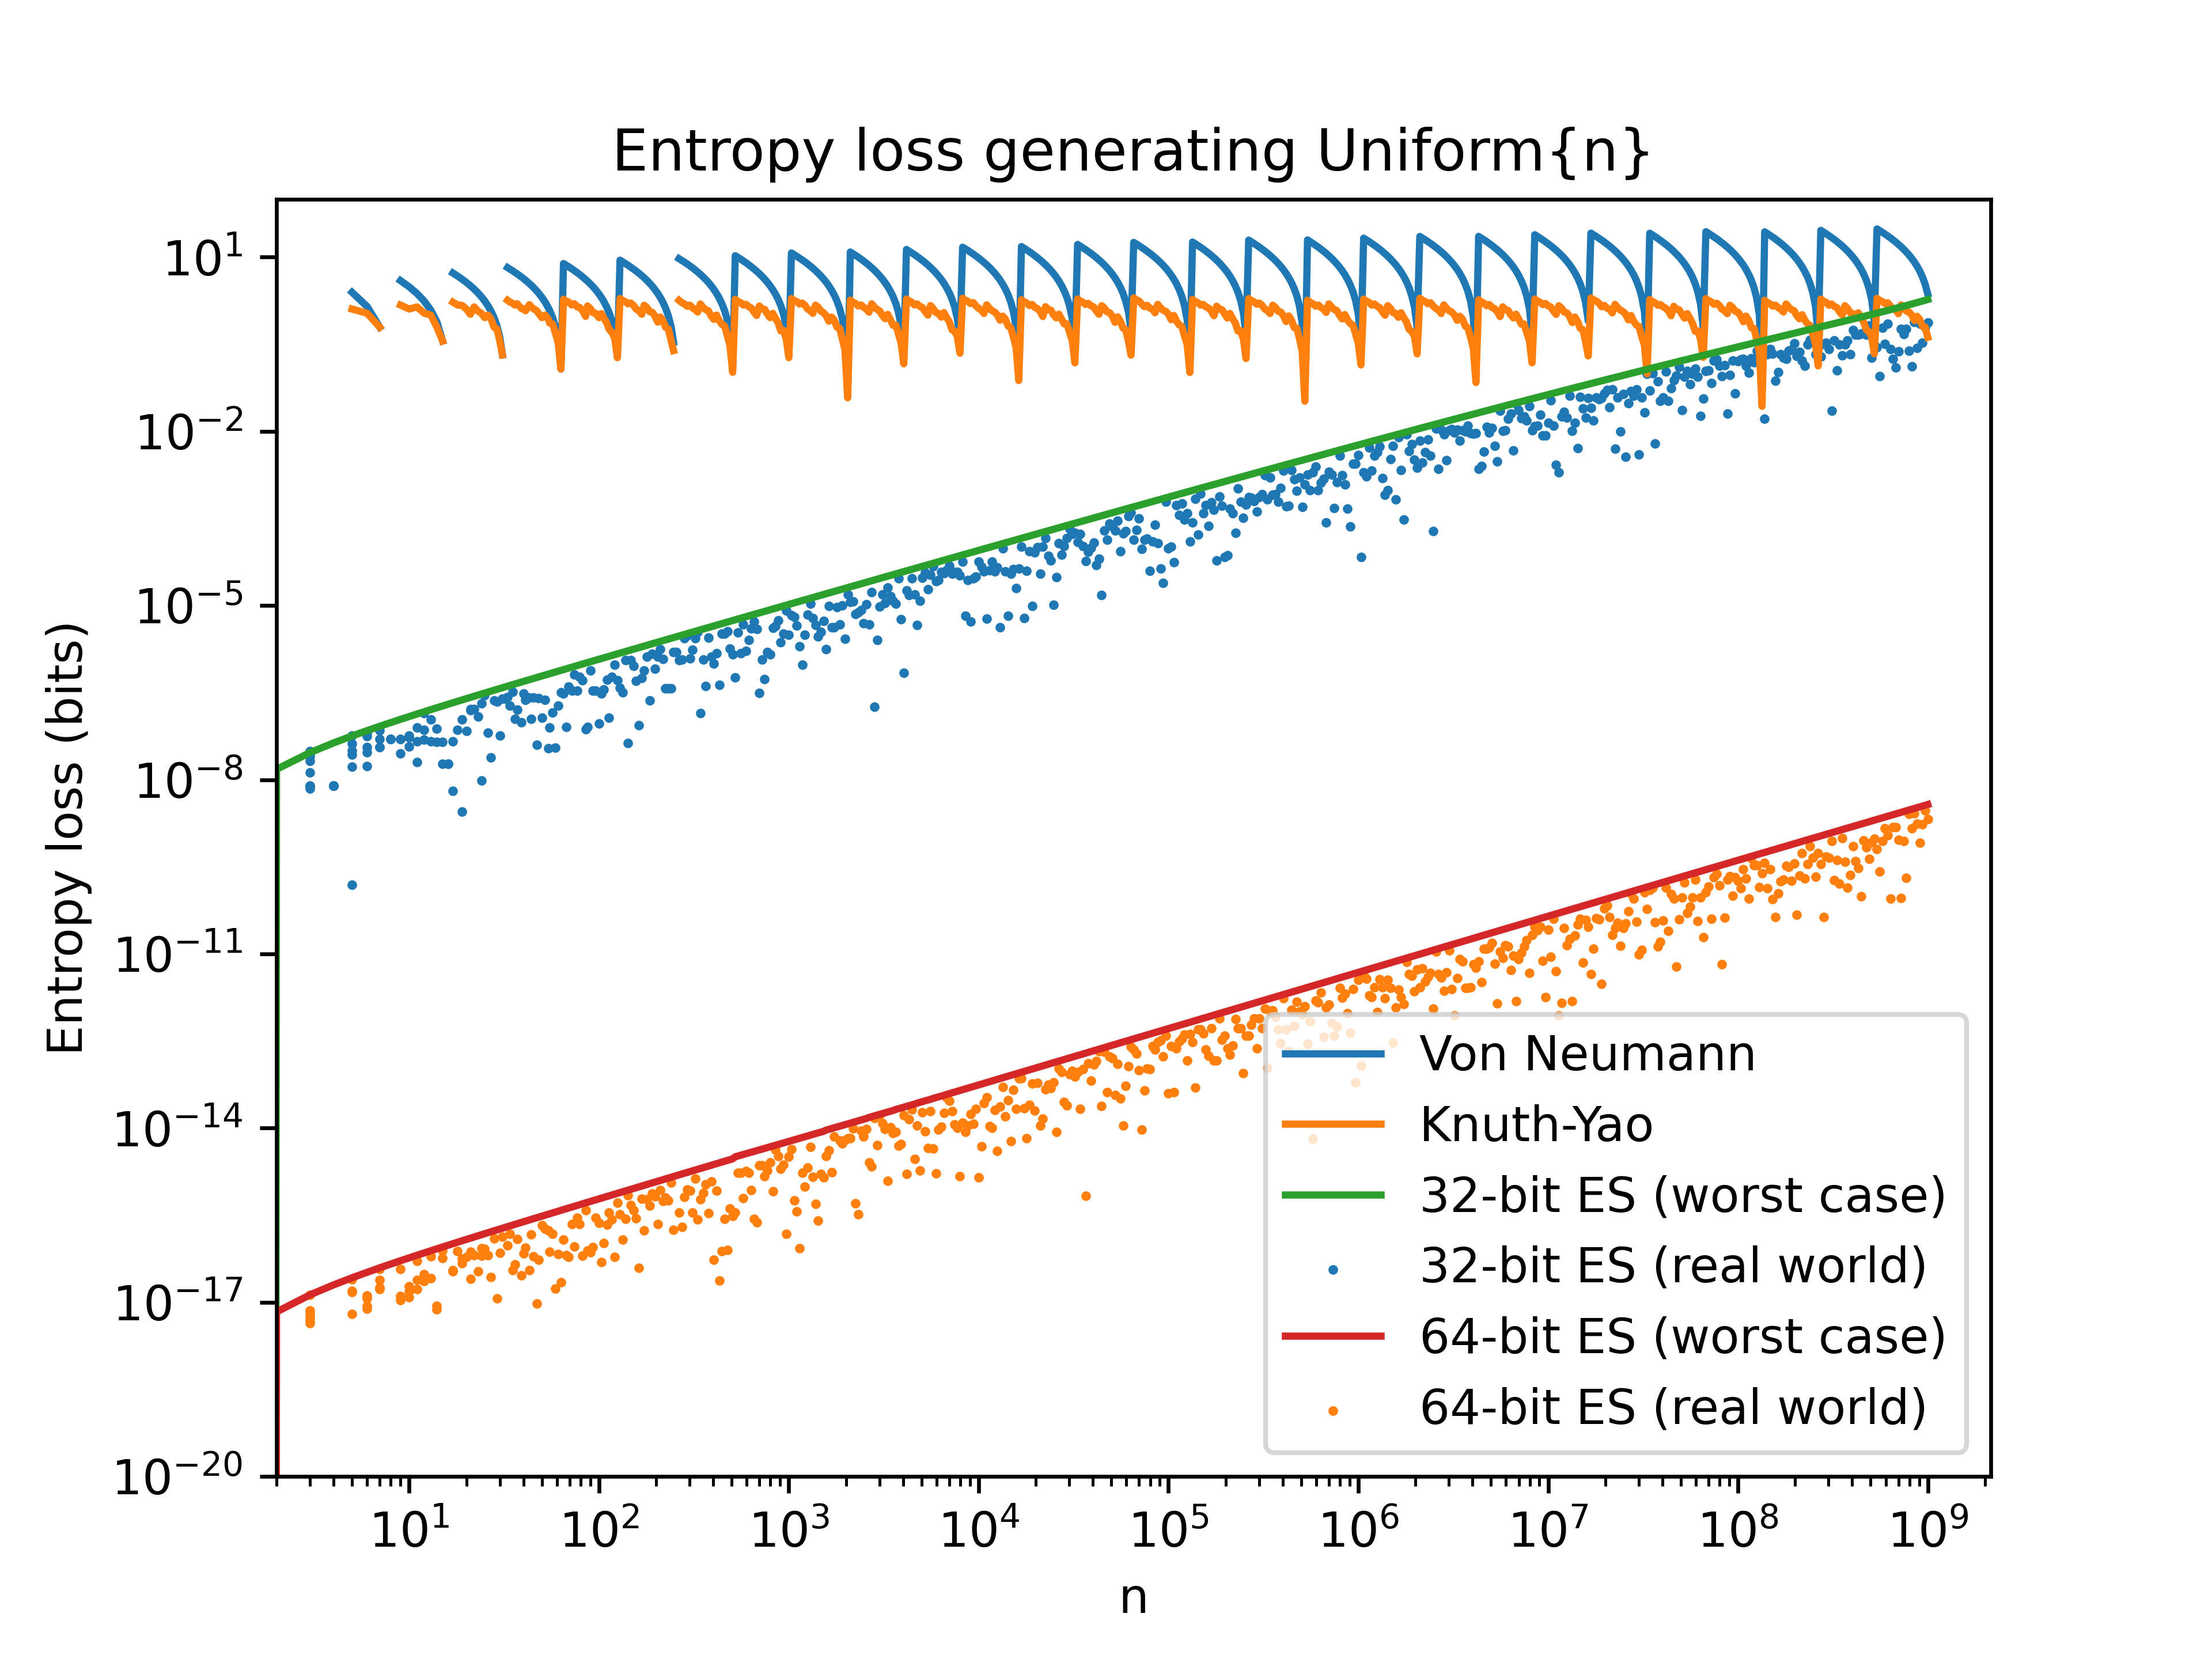
\includegraphics[width=0.8\textwidth]{uniform_losses.png}
\caption{Entropy losses for uniform variable generation.}
\label{fig:uniform-losses}
\end{figure}

Figure \ref{fig:shuffling-efficiency} shows the overall impact of entropy losses when applied to the shuffling a deck of $n$ cards using the Fisher-Yates algorithm \cite{fisher1953statistical, durstenfeld1964algorithm, knuth2014art}. This is a good demonstration of the entropy efficiency under a real-world workload. Calculations show that we can calculate that shuffling a deck of 52 cards can be done with an entropy loss of $\approxeq 1.7e-5$ bits, or an entropy efficiency of $\approxeq 0.99999992$.

\begin{figure}[ht]
\centering
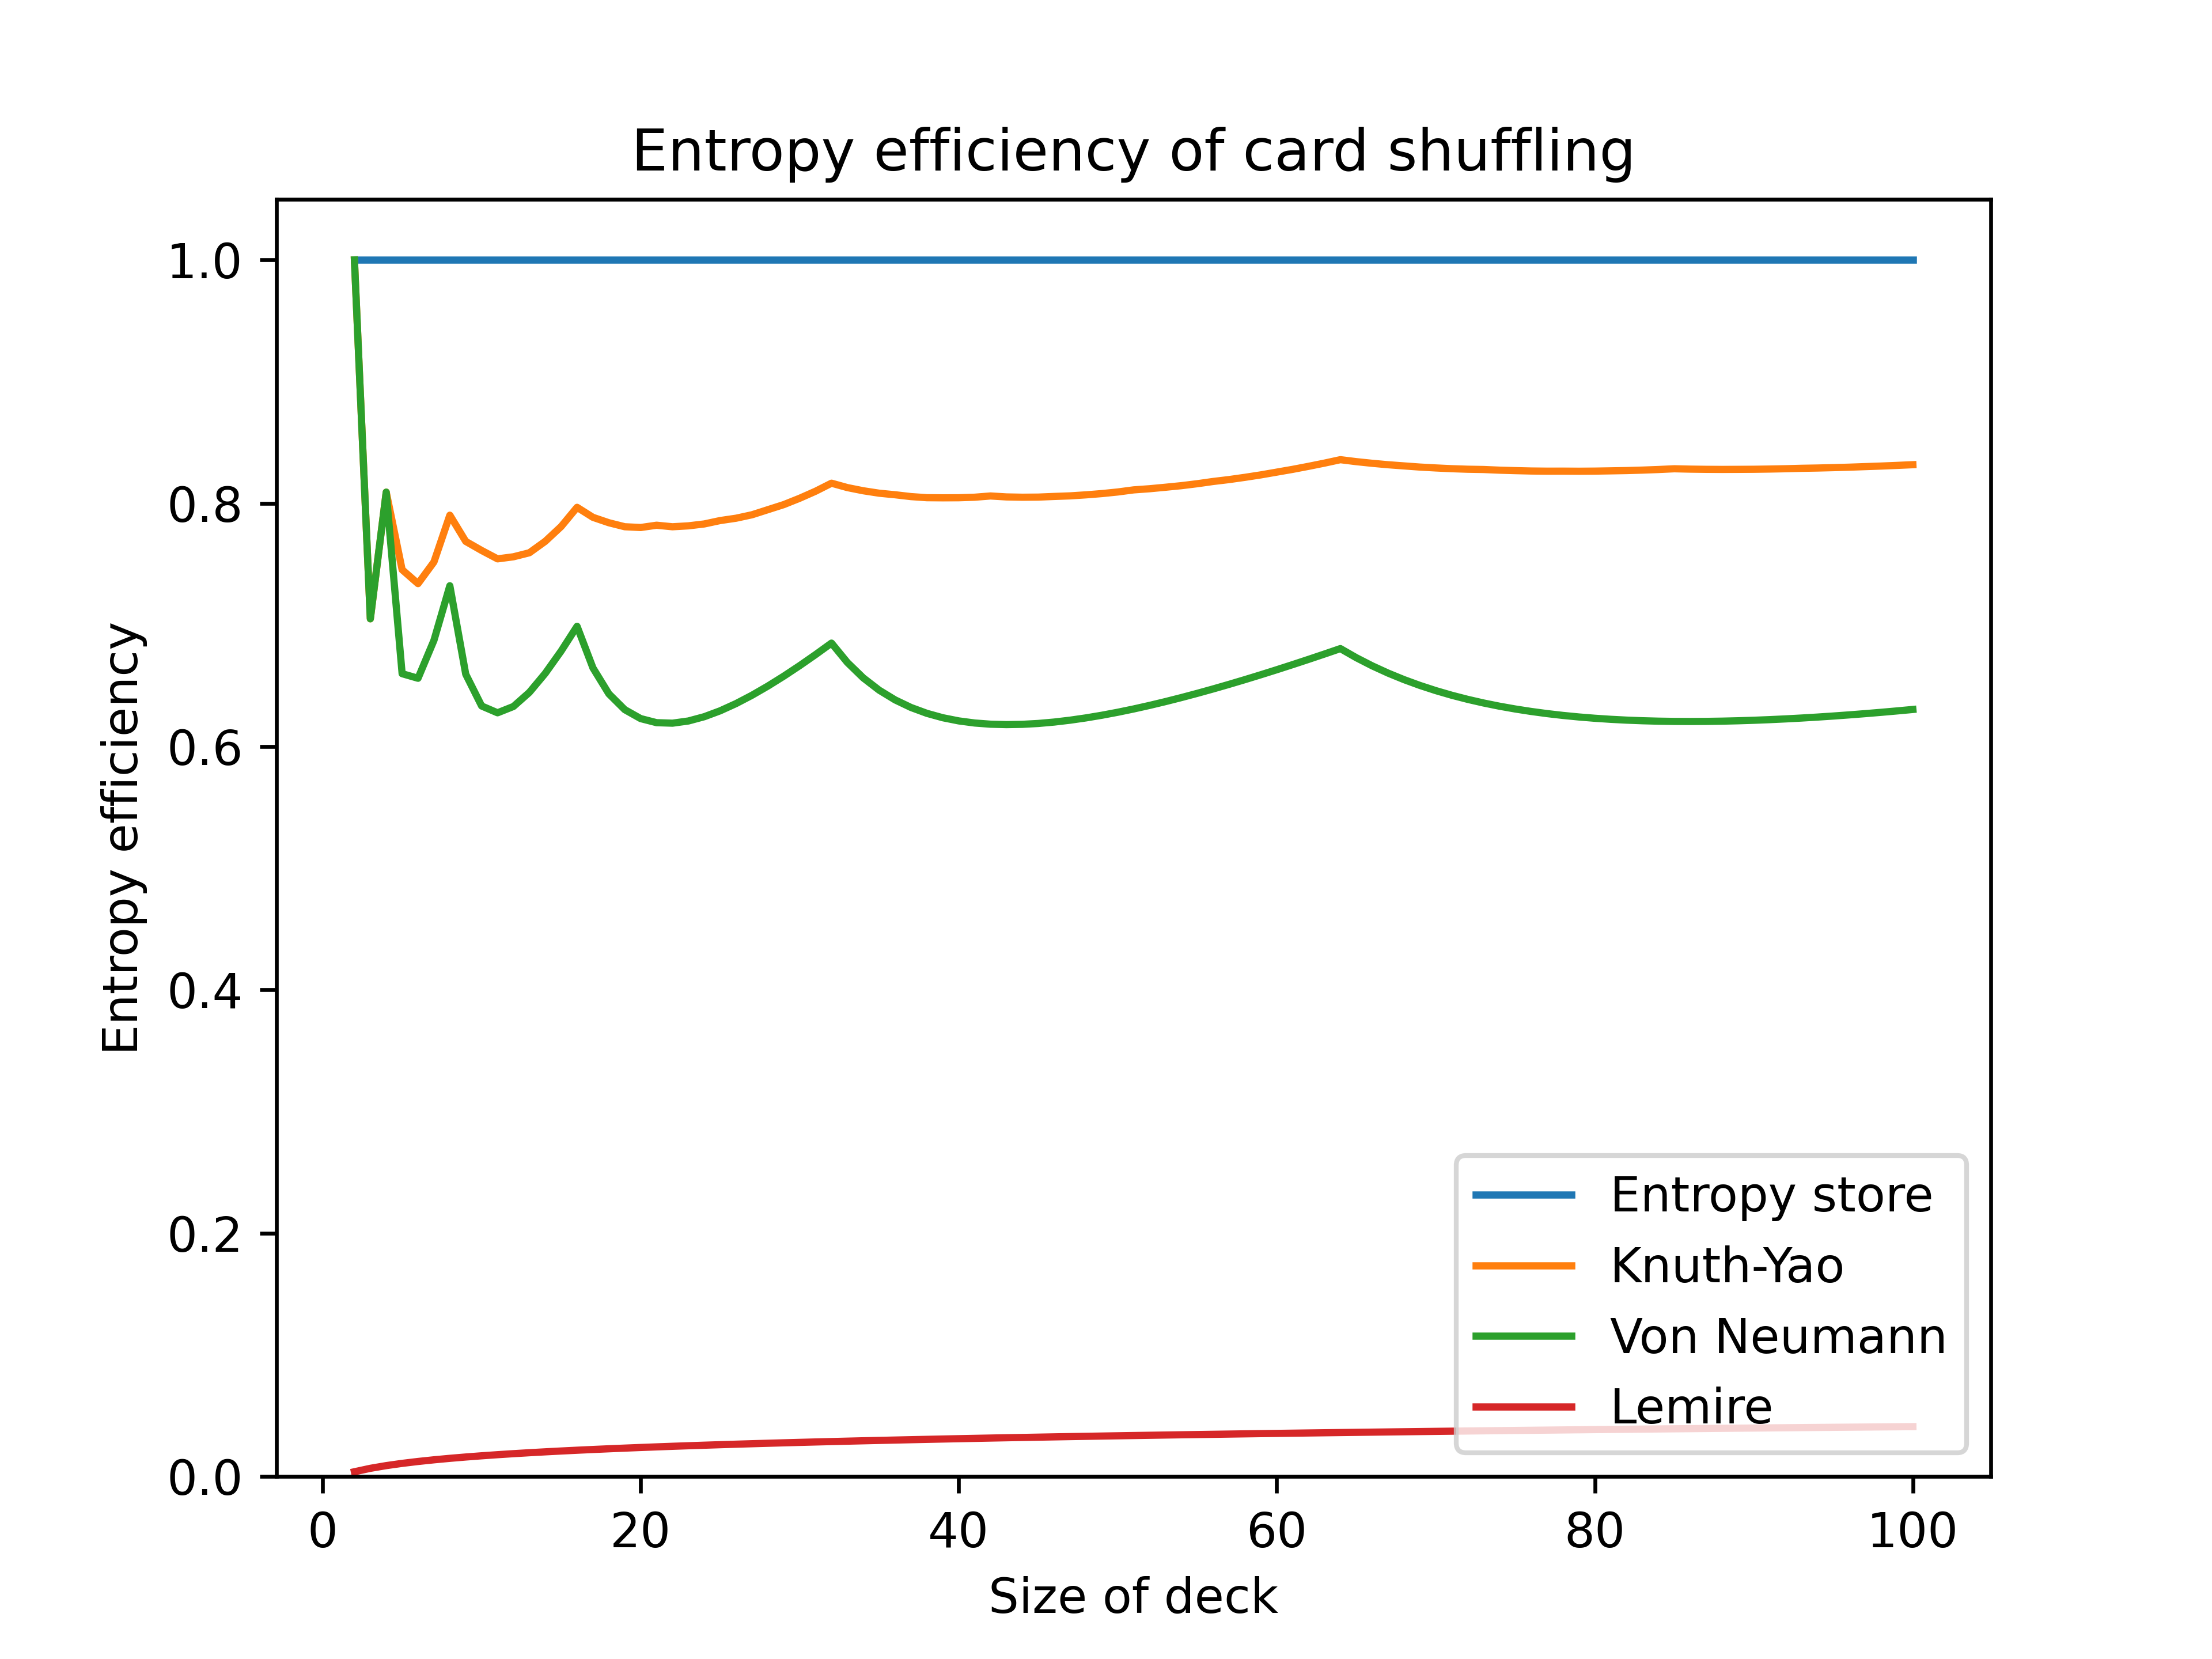
\includegraphics[width=0.8\textwidth]{shuffling_efficiency.png}
\caption{Entropy efficiency shuffling cards.}
\label{fig:shuffling-efficiency}
\end{figure}

When generating Bernoulli variables, we see in Figure \ref{fig:bernoulli-efficiency} that the entropy efficiency of the interval algorithm drops off significantly. IA must fetch between 1 and 2 bits per output on average. By contrast, ES algorithms to not necessarily fetch any bits to generate an output, as there may be enough entropy in the store already, so ES just shrinks the size of its store to generate an output. Figure \ref{fig:bernoulli-rate} shows that IA cannot significantly increase its output rate for low-entropy outputs.

\begin{figure}[ht]
\centering
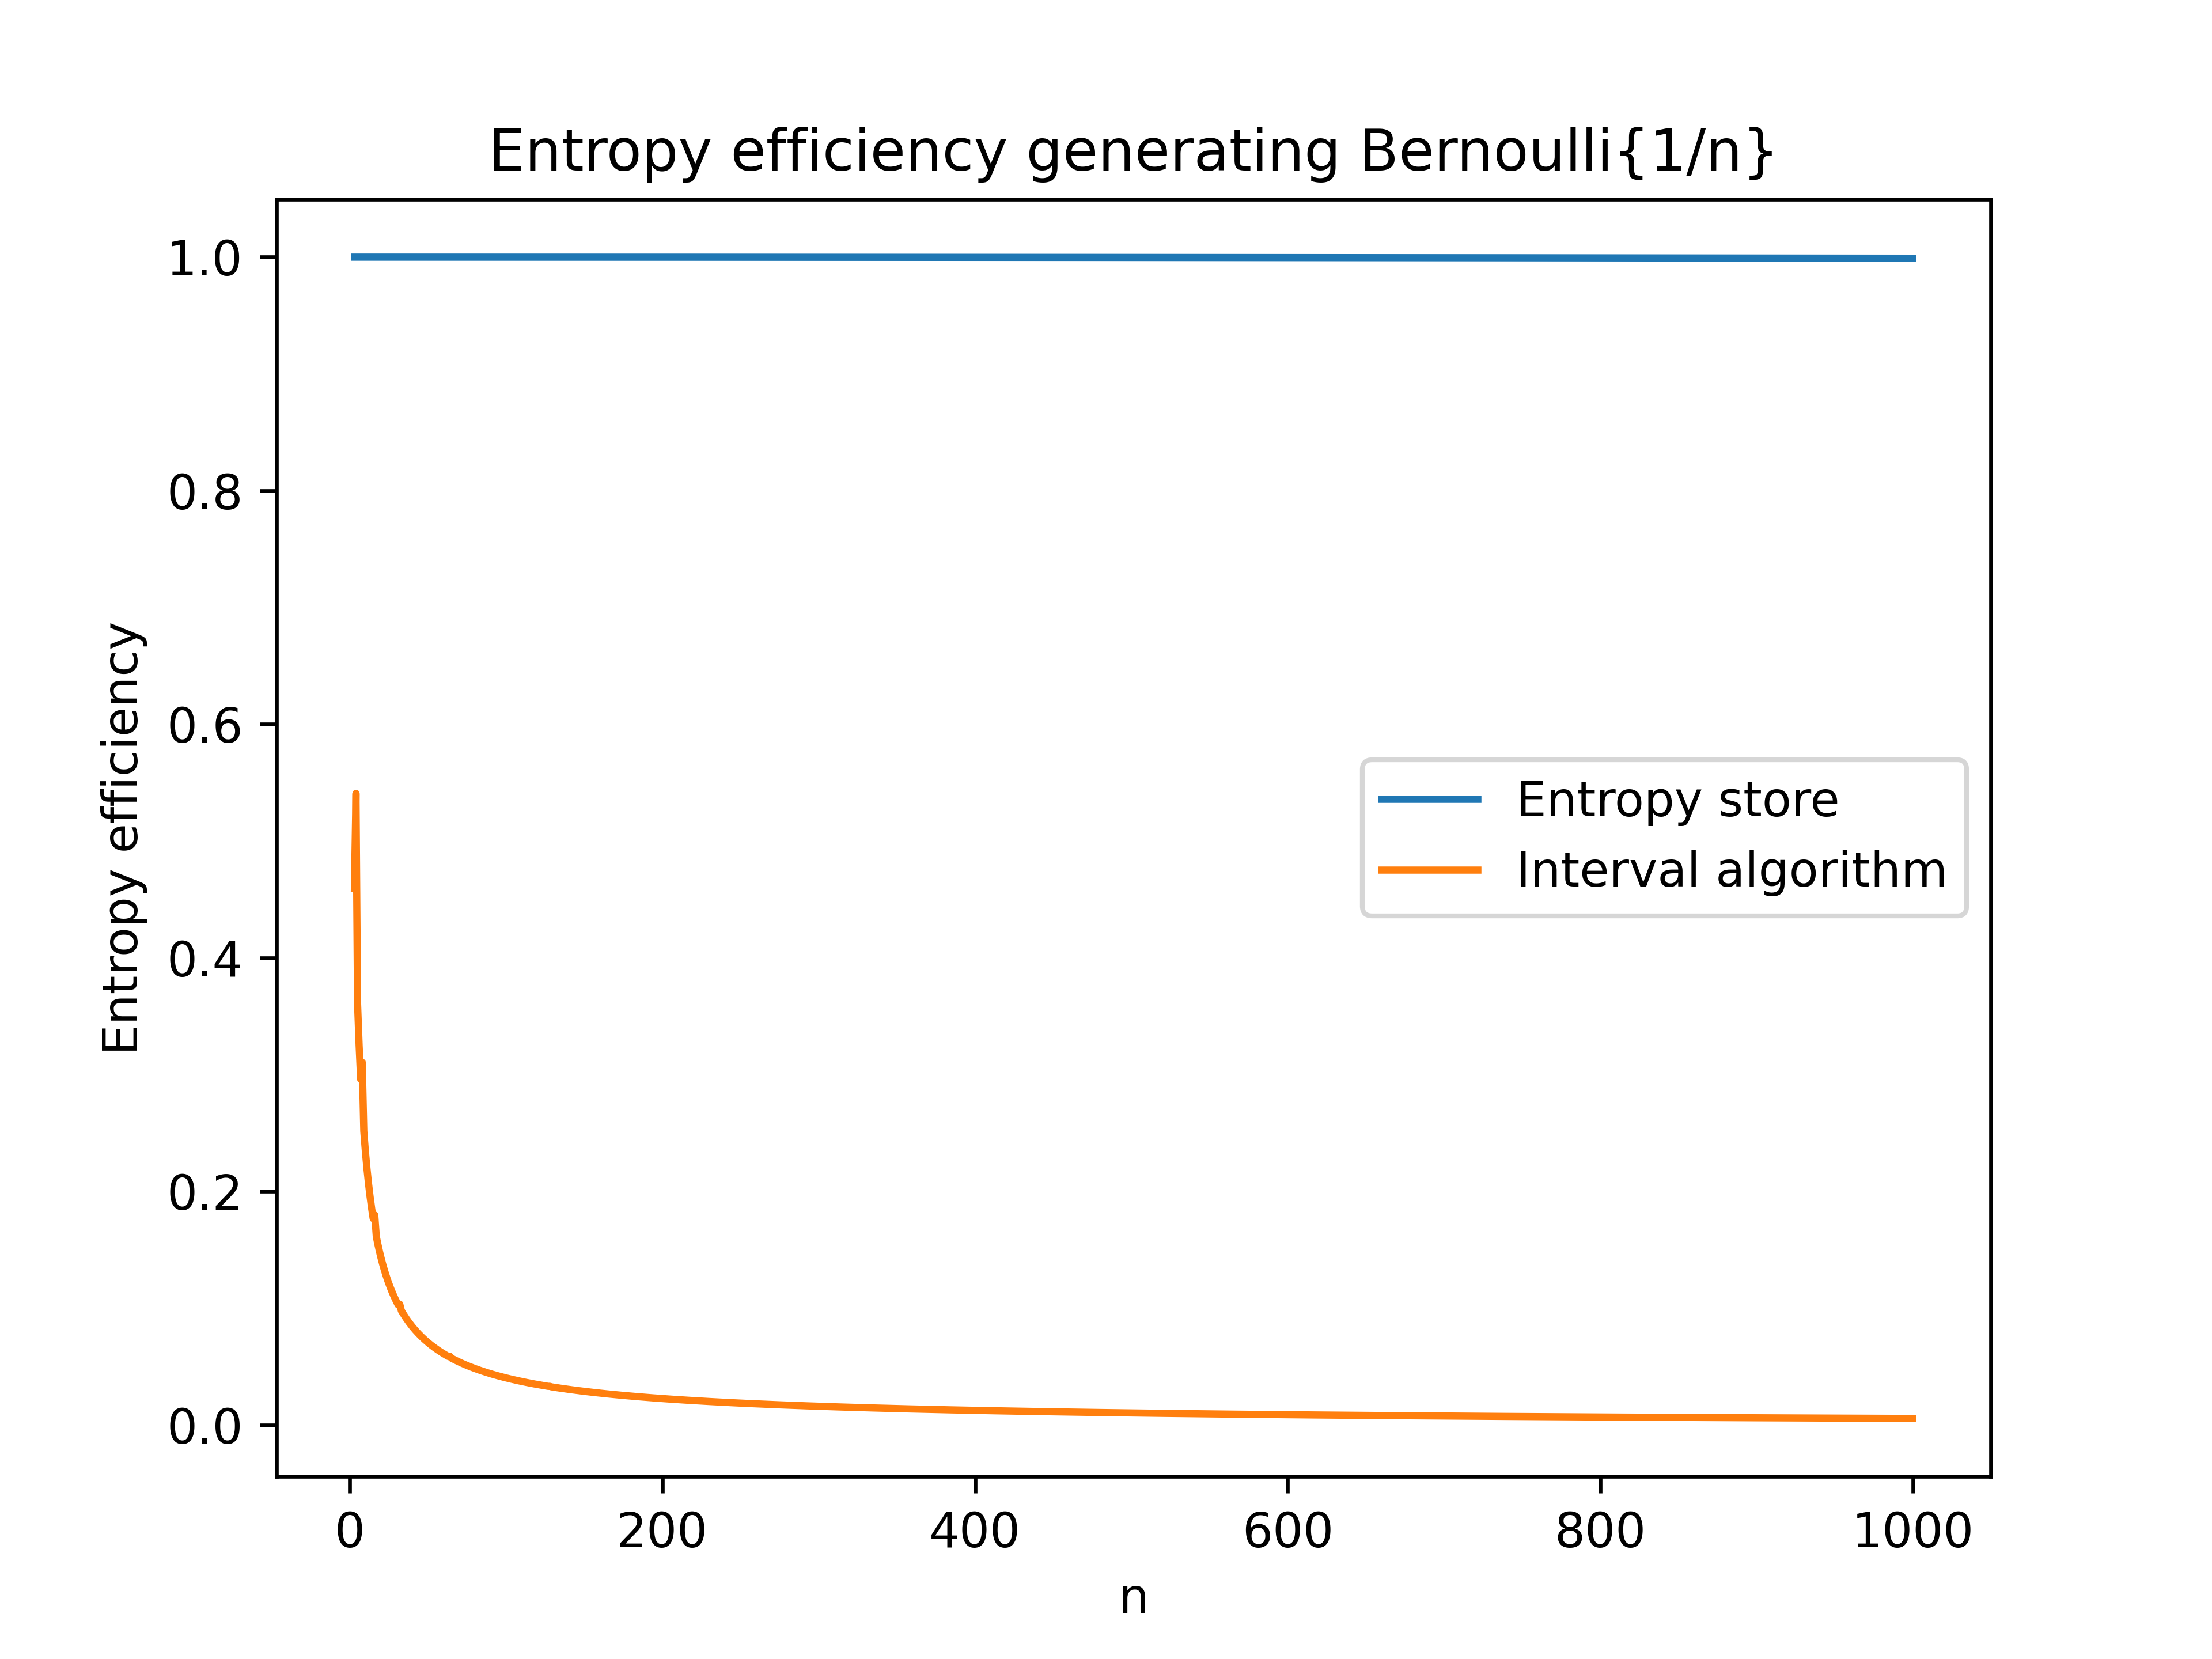
\includegraphics[width=0.8\textwidth]{bernoulli_efficiency.png}
\caption{Entropy efficiency generating Bernoulli variables.}
\label{fig:bernoulli-efficiency}
\end{figure}

\begin{figure}[ht]
\centering
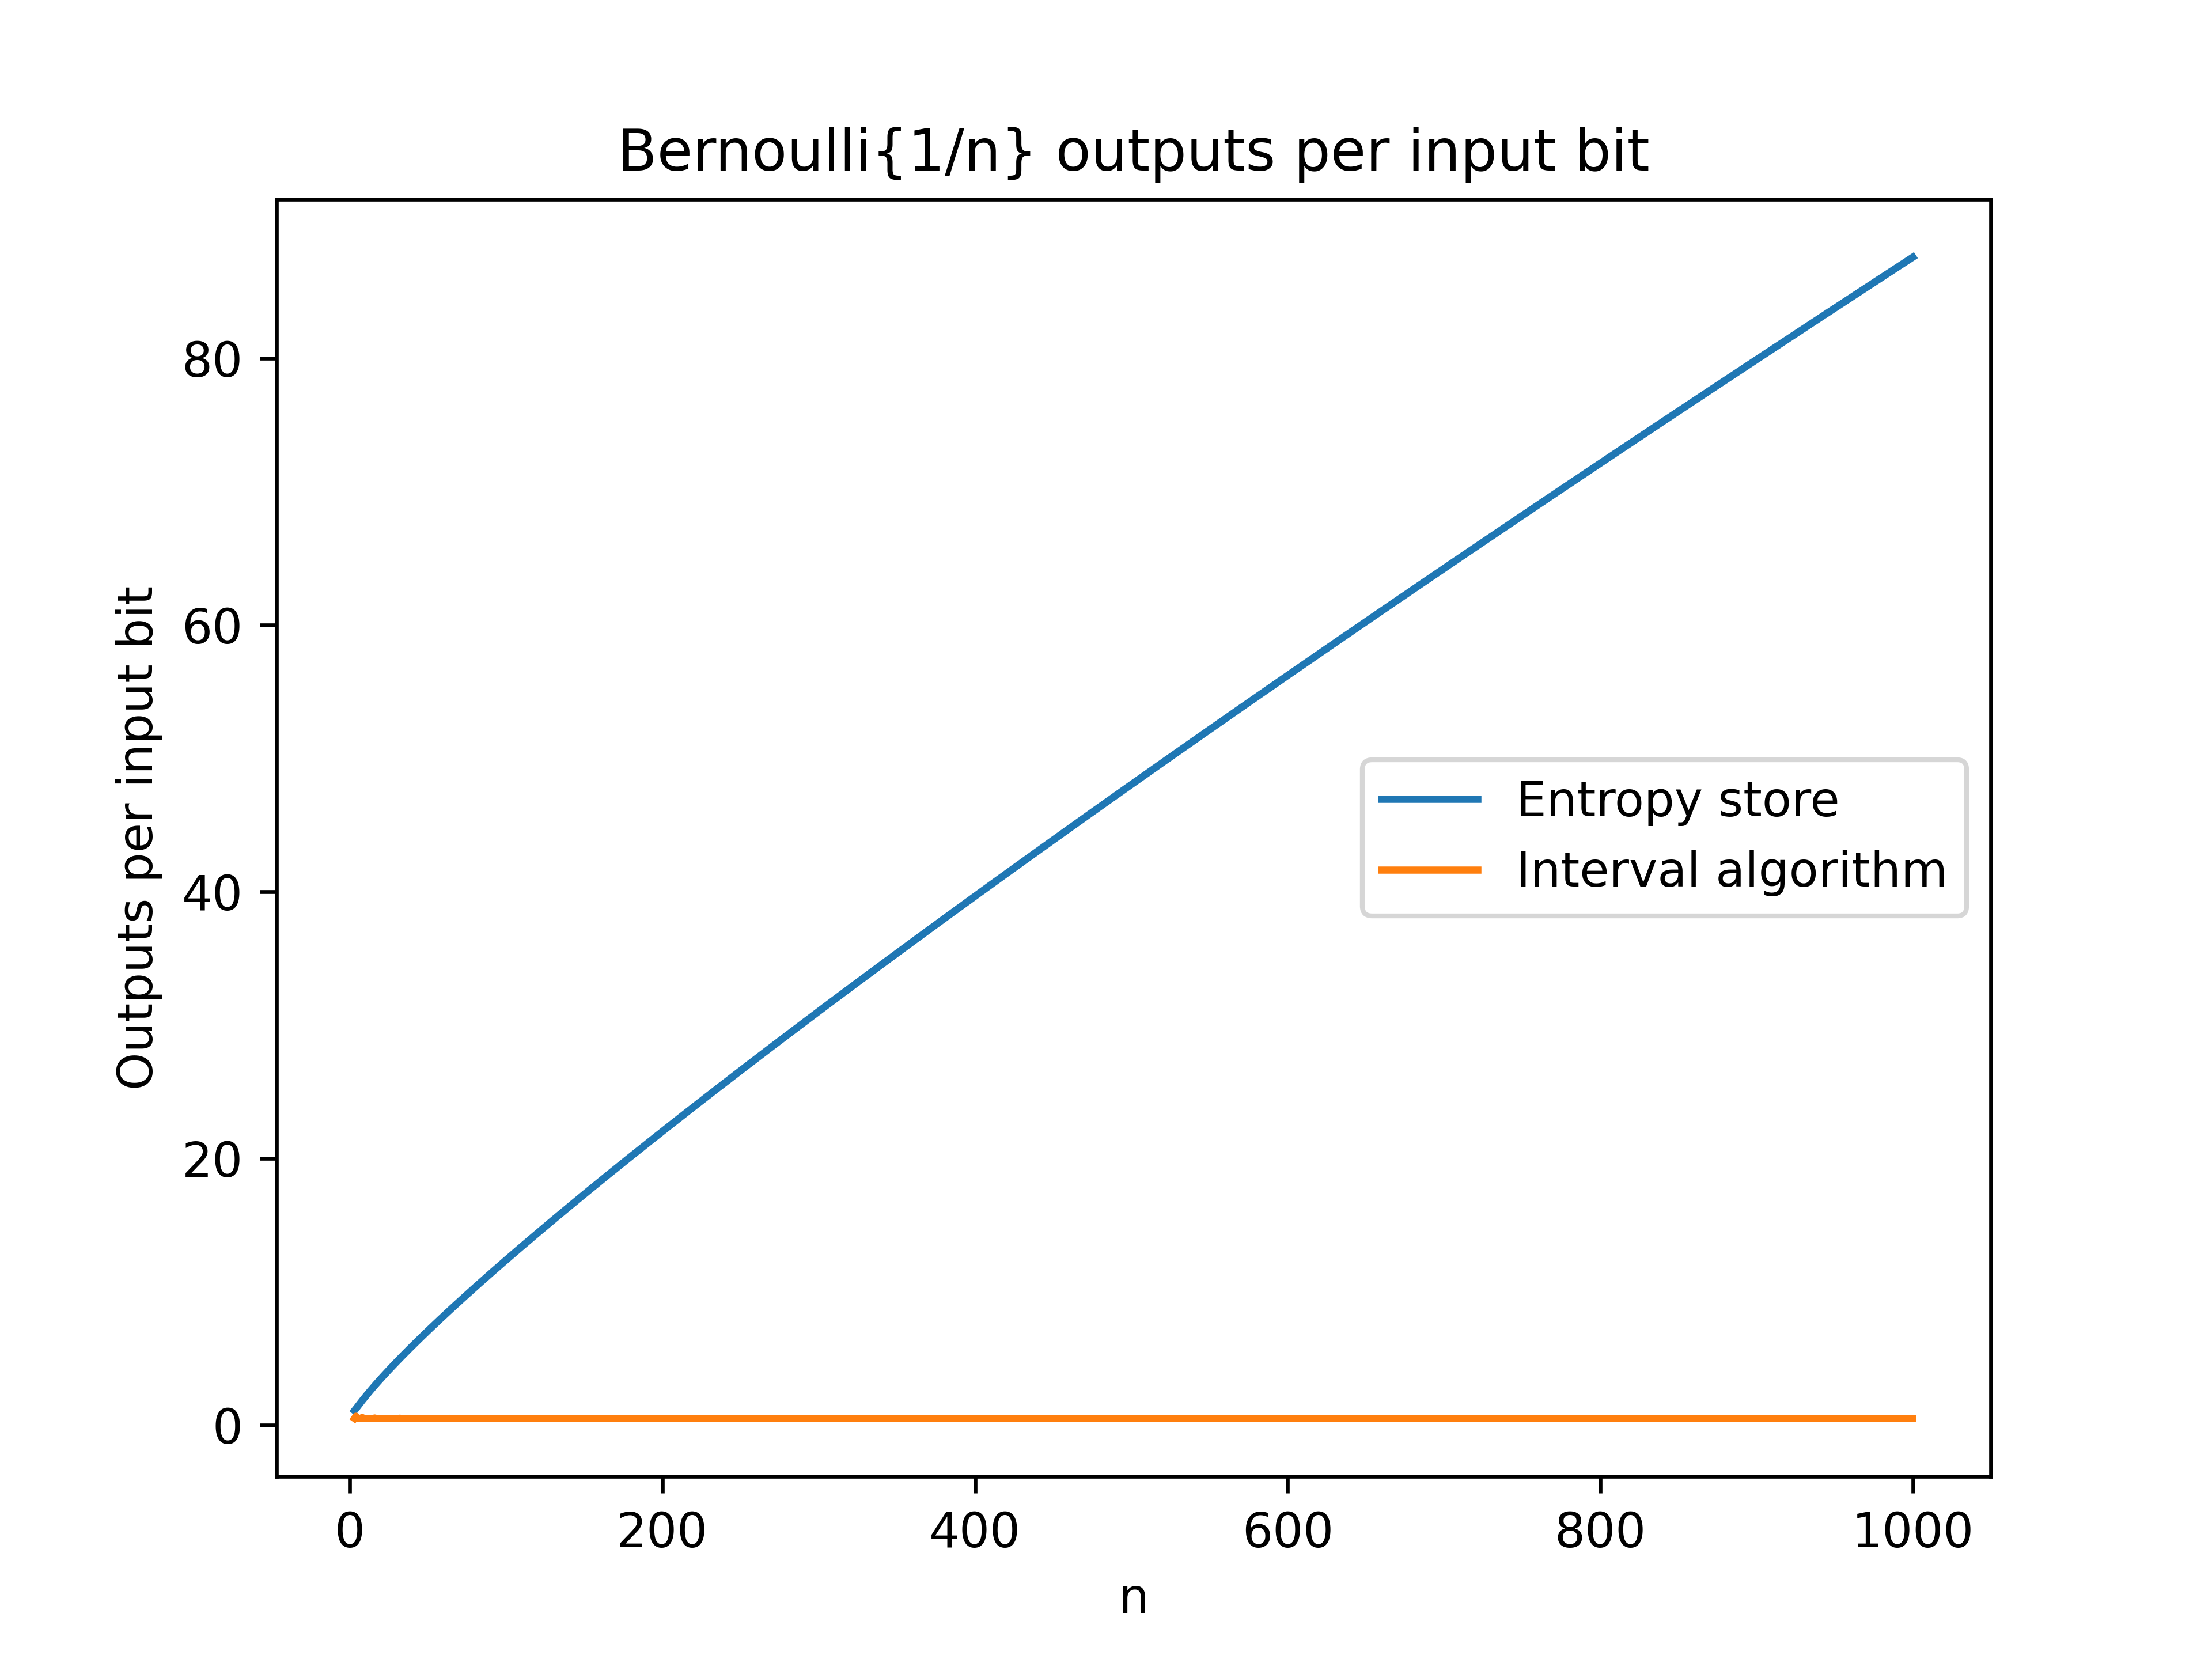
\includegraphics[width=0.8\textwidth]{bernoulli_rate.png}
\caption{Output rate for Bernoulli distributions.}
\label{fig:bernoulli-rate}
\end{figure}

Table~\ref{tab:speed} compares the speed of ES against various best in class random number generators. These numbers are heavily compiler and CPU dependent, so should only be considered a guide.

When reading entropy from a hardware random generator, rate of entropy input is the dominating factor and the ES is the fastest by a significant margin. When using a very fast pseudo-random source like Xorisho-128 \cite{blackman21}, we see that Lemire's algorithm \cite{lemire2019fast} dominates, as this is designed for speed and not entropy-efficiency.

Speed is best understood in terms of CPU pipeline architecture. Branching, memory access, hardware random numbers and integer divmod operations are all relatively expensive operations \cite{Abel19a}. Table-based methods like FLDR \cite{saad2020fldr} and ALDR \cite{saad2025} perform memory access which could be a bit slower than purely arithmetic methods. ES is likely to suffer due to its 2 integer divmod operations, but fortunately compilers can strength-reduce integer division to a multiplication and a shift \cite{granlund94}, which is shown in the "optimized" version of these algorithms in Table~\ref{tab:speed}. ES was fastest for Bernoulli outputs in all cases because there is actually one less division operation needed.

Overall, we can conclude that ES is most suited when generating truly random integers from a hardware entropy source. When a pseudo-random source is used, then Lemire's algorithm is the fastest. Using a 64-bit ES was not beneficial.

Integer division and multiplication is $O(n \log n)$ \cite{harvey2021integer}, for an $m$ bit buffer the complexity of ES is $O(m \log m)$, but for practical purposes it is $O(1)$ in time and space.

\begin{table}[h!]
\centering
\begin{tabular}{|c|c|c|c|}
\hline
Algorithm & Output & Hardware & Xoshiro-128++ \\
\hline
ES32                  & $Uniform\{6\}$ & 1 & 1 \\
ES32 optimized        & $Uniform\{6\}$ & 1 & 0.47 \\
ES64                  & $Uniform\{6\}$ & 1 & 1.24 \\
ES64 optimized        & $Uniform\{6\}$ & 1 & 0.55 \\
Von Neumann \cite{neumann51}     & $Uniform\{6\}$ & 1.55 & 0.77 \\
Fast Dice Roller \cite{lumbroso2013optimal} & $Uniform\{6\}$ & 1.42 & 0.83 \\
Huber-Vergas \cite{huber2024optimalrollingfairdice} & $Uniform\{6\}$ & 1.42 & 1.0 \\
FLDR \cite{saad2020fldr} & $Uniform\{6\}$ & 1.42 & 1.46 \\
ALDR \cite{saad2025} & $Uniform\{6\}$ & 1.42 & 1.5 \\
Lemire \cite{lemire2019fast} & $Uniform\{6\}$ & 24.8 & 0.26 \\
\hline

ES32                  & $Bernoulli\{\frac{1}{100}\}$ & 1 & 1 \\
ES32 optimized        & $Bernoulli\{\frac{1}{100}\}$ & 0.9 & 0.54 \\
FLDR                  & $Bernoulli\{\frac{1}{100}\}$ & 28.3 & 3.8 \\
ALDR                  & $Bernoulli\{\frac{1}{100}\}$ & 22.4 & 2.94 \\
Lemire (alias method) & $Bernoulli\{\frac{1}{100}\}$ & 700 & 1.07 \\

\hline

ES32                  & $Weighted\{1,2,3,4,5\}$ & 1 & 1 \\
FLDR                  & $Weighted\{1,2,3,4,5\}$ & 1.36 & 1.38 \\
ALDR                  & $Weighted\{1,2,3,4,5\}$ & 1.36 & 1.13 \\
Lemire (alias method) & $Weighted\{1,2,3,4,5\}$ & 29.8 & 0.18 \\

\hline

\end{tabular}
\caption{Relative times generating integers from different binary entropy sources (lower is better).}
    \label{tab:speed}
\end{table}



\section{Conclusion}

We have introduced a new class of algorithm to generate random integers via a uniform entropy store, and shown that by recycling unused entropy between outputs we can achieve arbitrarily low entropy losses. We have shown that the entropy efficiency limits of classical algorithms like Knuth-Yao and the Interval Algorithm can be overcome by using an entropy store. 

A big benefit of ES is that no setup step is needed for uniform and Bernoulli outputs, and that the same ES can be shared between different output types. ES is fastest when generating outputs from a hardware entropy source and for Bernoulli outputs, but is still competitive on pseudorandom entropy sources, particularly if the division operations can be optimized.



\printbibliography

\appendix

\section {Source code} \label{app:source-code}

Source code for $generate\_uniform$, written in C.

\begin{verbatim}
    const uint32_t s_min = 1<<31;
    uint32_t s_value = 0, s_range = 1;

    uint32_t generate_uniform32(uint32_t n)
    {
        for(;;)
        {
            // Preload entropy one bit at a time into s
            while(s_range < s_min)
            {
                s_value <<= 1;
                s_value |= fetch();
                s_range <<= 1;
            }
            // Sample entropy s to a multiple of n
            uint32_t r = s_range / n;
            uint32_t c = s_range % n;
            if(s_value >= c)
            {
                // Sample successful
                s_value -= c;
                uint32_t a = s_value / n;
                uint32_t b = s_value % n;
                s_value = a;
                s_range = r; 
                return b;
            }
            else
            {
                // Reject
                s_range = c;
            }
        }
    }
\end{verbatim}

\end{document}
